\documentclass[10pt,a4paper]{article}

% ── Packages ───────────────────────────────────────────────────────────
\usepackage[utf8]{inputenc}
\usepackage[T1]{fontenc}
\usepackage{lmodern}
\usepackage{microtype}
% lmodern ships no bold small-caps in T1; fall back to medium small-caps so that
% \textsc{...} inside bold headers renders cleanly (silences the substitution warning).
\DeclareFontShape{T1}{lmr}{bx}{sc}{<->ssub*lmr/m/sc}{}
\usepackage{amsmath,amssymb,amsfonts}
\usepackage{graphicx}
\usepackage{xcolor}
\usepackage{booktabs}
\usepackage{multirow}
\usepackage{array}
\usepackage{hyperref}
\usepackage{listings}
\usepackage{caption}
\usepackage{subcaption}
\usepackage{enumitem}
\usepackage{fancyhdr}
\usepackage{lastpage}
\usepackage{geometry}
\usepackage{algorithm}
\usepackage{algpseudocode}
\usepackage{tikz}
\usetikzlibrary{shapes,arrows,positioning,calc,fit,backgrounds}
\usepackage{pgfplots}
\pgfplotsset{compat=1.18}

% ── Page geometry ────────────────────────────────────────────────────────
\geometry{
  left=2.5cm, right=2.5cm,
  top=2.5cm, bottom=2.5cm,
  headheight=14pt
}

% ── Colors ───────────────────────────────────────────────────────────────
\definecolor{swlpblue}{HTML}{2874A6}
\definecolor{airllmorange}{HTML}{E67E22}
\definecolor{ssdblue}{HTML}{1A5276}
\definecolor{ramgreen}{HTML}{1E8449}
\definecolor{mpsbrown}{HTML}{784212}
\definecolor{lightgray}{HTML}{F5F5F5}
\definecolor{medgray}{HTML}{CCCCCC}
\definecolor{codebg}{HTML}{F8F8F8}

% ── Hyperref setup ─────────────────────────────────────────────────────
\hypersetup{
  colorlinks=true,
  linkcolor=swlpblue,
  citecolor=swlpblue,
  urlcolor=swlpblue,
  pdftitle={SWLP: Sliding Window Layer Pipeline for Lossless LLM Inference on Consumer Hardware},
  pdfauthor={Rishav Upadhaya},
  pdfsubject={Memory-efficient LLM inference via weight streaming},
  pdfkeywords={LLM inference, weight streaming, Apple Silicon, NVMe offload, consumer hardware}
}

% ── Code listings ────────────────────────────────────────────────────────
\lstset{
  backgroundcolor=\color{codebg},
  basicstyle=\ttfamily\small,
  breaklines=true,
  frame=single,
  rulecolor=\color{medgray},
  showstringspaces=false,
  keywordstyle=\color{swlpblue}\bfseries,
  commentstyle=\color{gray}\itshape
}

% ── Header/Footer ────────────────────────────────────────────────────────
\pagestyle{fancy}
\fancyhf{}
\fancyhead[L]{\small\textit{SWLP: Lossless LLM Inference via Weight Streaming}}
\fancyhead[R]{\small\thepage\ of \pageref{LastPage}}
\renewcommand{\headrulewidth}{0.4pt}

% ── Custom commands ──────────────────────────────────────────────────────
\newcommand{\swlp}{\textsc{swlp}}
\newcommand{\etal}{\textit{et al.}}
\newcommand{\ie}{\textit{i.e.}}
\newcommand{\eg}{\textit{e.g.}}
\newcommand{\wrt}{\textit{w.r.t.}}

% ── Bibliography note ────────────────────────────────────────────────────
% This document ships a self-contained `thebibliography' environment so it
% compiles on the arXiv AutoTeX servers from a single .tex file with no
% external .bib/.bbl dependency (the most robust submission path). A matching
% references.bib is provided alongside this file; to use BibTeX instead, remove
% the thebibliography block at the end and replace it with:
%     \bibliographystyle{IEEEtran}
%     \bibliography{references}
% then compile pdflatex -> bibtex -> pdflatex -> pdflatex and upload the .bbl.

% ── Title metadata ───────────────────────────────────────────────────────
\title{
  \textbf{SWLP: Sliding Window Layer Pipeline}\\[0.3em]
  \large Characterizing Lossless FP16 LLM Inference on Apple Silicon Unified Memory
}
\author{
  Rishav Upadhaya\\
  \textit{Independent Researcher}\\
  \texttt{rishavupadhaya266@gmail.com}
}
\date{June 2026}

% ═══════════════════════════════════════════════════════════════════════════
% DOCUMENT BEGINS
% ═══════════════════════════════════════════════════════════════════════════
\begin{document}

\maketitle
\thispagestyle{fancy}

% ── Abstract ─────────────────────────────────────────────────────────────
\begin{abstract}
Running large language models that exceed device memory by streaming weights from
storage is a well-established technique (ZeRO-Inference, FlexGen, LLM in a Flash,
AirLLM, oLLM), but almost all of it targets NVIDIA CUDA GPUs with discrete VRAM.
We study the technique on a different and increasingly common platform, Apple
Silicon \textbf{unified memory}, where RAM and GPU memory are one pool and the
OS page cache competes directly with the model's working set. We implement
lossless FP16 layer streaming on PyTorch/MPS (\swlp) and make three contributions.
\textbf{(1)~Characterization:} we measure \swlp{} across model scales (7B--24B) on a
16~GB M5, reporting throughput, latency, and peak memory, and isolating where
unified memory behaves differently from discrete VRAM (\eg, the macOS
memory-compressor cliff when resident layers starve the page cache).
\textbf{(2)~A reproducible protocol:} we show that a warm OS page cache silently
inflates streaming throughput by reading from RAM rather than storage, enough
to exceed the cold-storage physical ceiling, and provide a cold/warm protocol
with per-run provenance that prevents this error, documenting a concrete instance
of a physically impossible reported result. \textbf{(3)~A feasibility boundary:}
from the bound $\text{tok/s} \le \text{SSD}_{\text{bw}} / \text{model}_{\text{bytes}}$
and our measurements, including two negative results (FP8 storage and in-RAM
residency), we show that single-stream, lossless, interactive inference of
larger-than-RAM models is over-constrained: no scheduling improvement can cross
the bandwidth bound. On an Apple M5 (16~GB unified memory, 6.93~GB/s NVMe), \swlp{}
runs Mistral-7B FP16 at \textbf{0.174~tok/s cold-cache} and 0.21~tok/s warm-cache
with a \textbf{1.21~GB} peak footprint; even cold, it achieves
\textbf{2.05$\times$ the throughput of warm AirLLM~2.11.0}. A 44~GB Mistral-Small-24B
that cannot load at all under naive inference runs at 0.081~tok/s in 3.76~GB RAM.
\swlp{} is open source; install from source (Appendix~\ref{app:reproduction}).
\end{abstract}

\textbf{Keywords:} large language model inference, weight streaming,
memory-efficient inference, Apple Silicon, unified memory, NVMe offload,
reproducible benchmarking, consumer hardware

\vspace{1em}
\hrule
\vspace{1em}

% ── Front matter ends ─────────────────────────────────

% ═══════════════════════════════════════════════════════════════════════════
% I. INTRODUCTION
% ═══════════════════════════════════════════════════════════════════════════
\section{Introduction}
\label{sec:intro}

\subsection{Motivation}
\label{subsec:motivation}

The proliferation of open-weight large language models (LLMs) such as Mistral-7B
\cite{jiang2023mistral}, Llama-3 \cite{llama32024}, and Qwen2.5 \cite{qwen2024}
has created a gap between model capability and hardware accessibility. A
full-precision (FP16) Mistral-7B checkpoint occupies 13.96~GB; Mistral-Small-24B
requires 44~GB. A typical consumer laptop has 16~GB of RAM. The model simply does
not fit.

Existing solutions trade quality for feasibility. GPTQ \cite{frantar2023gptq},
AWQ \cite{lin2023awq}, and llama.cpp GGUF \cite{gerganov2023llama} apply weight
quantization, introducing rounding error at every layer. These reduce storage by
2--8$\times$ but alter the model's numeric outputs. For research reproducibility,
perplexity and sensitivity analysis, or applications requiring deterministic
outputs, lossless FP16 inference remains a hard requirement.

\swlp{} (Sliding Window Layer Pipeline) makes the opposite trade-off: \emph{pay
in latency, not in quality}. A transformer's forward pass is strictly sequential
(layer $i$ must complete before layer $i+1$ starts), so only the layers
currently computing need to reside in RAM; the rest stay on the SSD. A background
thread prefetches $W$ layers ahead, so SSD reads are largely hidden behind
compute. The novelty of this paper is not the mechanism (which is credited to
prior work) but a careful empirical \emph{characterization} of it on a platform
the literature has largely ignored: Apple Silicon unified memory.

\subsection{Research Questions}
\label{subsec:rq}

This work is organized around four research questions, each answered empirically
in Section~\ref{sec:results}:

\begin{description}[leftmargin=2.2em,style=nextline]
  \item[\textbf{RQ1}] Can lossless FP16 models that exceed unified memory be run
    on consumer Apple Silicon by streaming weights, and at what throughput,
    latency, and peak-memory cost across scales (7B, 14B, 24B)?
    (\S\ref{subsec:ladder})
  \item[\textbf{RQ2}] How does Apple Silicon \emph{unified} memory differ from
    discrete VRAM for weight streaming, specifically: does the shared
    RAM/page-cache pool create failure modes (memory compressor, residency
    cliffs) absent on CUDA? (\S\ref{subsec:residency}, \S\ref{sec:discussion})
  \item[\textbf{RQ3}] What throughput is achievable relative to the
    storage-bandwidth ceiling $\text{tok/s}\le B/M$, and can scheduling or
    precision tricks (prefetch depth $W$, FP8 storage, in-RAM residency)
    move it? (\S\ref{subsec:window}, \S\ref{subsec:residency}, \S\ref{subsec:fp8})
  \item[\textbf{RQ4}] How does \swlp{} compare to the closest lossless-streaming
    baseline (AirLLM) in throughput, latency, peak memory, and architecture
    coverage, under a cache-controlled protocol? (\S\ref{subsec:throughput}--\S\ref{subsec:cold})
\end{description}

\subsection{Contributions}
\label{subsec:contrib}

\begin{enumerate}[leftmargin=2em]
  \item \textbf{A systematic empirical characterization of lossless FP16 weight
    streaming on Apple Silicon unified memory.} To our knowledge, a clean
    PyTorch/MPS FP16 characterization across 7B/14B/24B has not been previously
    reported; prior art targets CUDA/discrete VRAM (ZeRO, FlexGen) or uses
    sparsity and custom stacks on Apple (LLM in a Flash). We measure throughput,
    TTFT, and peak RAM for three model scales and relate each to its
    bandwidth ceiling.

  \item \textbf{The page-cache measurement pitfall and a protocol that prevents
    it.} We show the warm-vs-cold gap empirically, document an impossible-number
    case study (a reported 0.505~tok/s above the 0.496~tok/s cold ceiling), and
    provide a provenance-stamped \texttt{--cold} protocol. This is a methods
    contribution the offloading literature under-reports.

  \item \textbf{A feasibility boundary for single-stream lossless streaming,
    including negative results.} We combine the bandwidth bound with measured
    overhead to map the precision$\times$latency$\times$feasibility surface. We
    report two negative results as first-class findings: FP8 storage does not
    help under per-token re-materialization, and in-RAM residency does not help
    on 16~GB. Both delimit the design space.

  \item \textbf{A multi-baseline reproduction harness.} \swlp{} and AirLLM are
    measured head-to-head under one cold/warm protocol with per-run provenance.
    HF~Accelerate disk-offload and CUDA adapters (oLLM, ZeRO-Inference) are
    \emph{implemented} in the harness but not yet benchmarked; the empirical
    evaluation in this version is Apple-Silicon-only and these paths are deferred
    to future work (Section~\ref{sec:limitations}).
\end{enumerate}

\textbf{What is not claimed.} We do not claim a novel algorithm, a new scheduler,
or a speed record. The prefetch/window/eviction mechanics are credited to prior
work in Section~\ref{sec:related}; the framing is ``we implement the standard
technique on a new platform and measure it carefully.''

% ═══════════════════════════════════════════════════════════════════════════
% II. RELATED WORK
% ═══════════════════════════════════════════════════════════════════════════
\section{Related Work}
\label{sec:related}

Table~\ref{tab:related} positions \swlp{} against the most relevant systems along
the three axes that matter for this paper: whether the method is lossless, the
target hardware, and its key limitation relative to consumer Apple Silicon.

\begin{table}[htbp]
\centering
\caption{Positioning of \swlp{} relative to prior weight-streaming and
compression work}
\label{tab:related}
\small
\begin{tabular}{@{}p{2.6cm}p{3.3cm}cp{3.6cm}@{}}
\toprule
\textbf{System} & \textbf{Approach} & \textbf{Lossless} & \textbf{Limitation \wrt{} our setting} \\
\midrule
GPTQ / AWQ \cite{frantar2023gptq,lin2023awq} & Post-training INT4/INT8 quantization & No & Alters numeric outputs \\
llama.cpp GGUF \cite{gerganov2023llama} & Quantized Metal kernels & No & Lossy; quant-only \\
AirLLM \cite{guo2023airllm} & Layer load$\to$\allowbreak compute$\to$\allowbreak discard (MLX) & Yes & Higher resident RAM; fails on explicit \texttt{head\_dim} \\
LLM in a Flash \cite{alizadeh2023llmflash} & Sparsity + flash loading & No & Needs ReLU sparsity; Apple-internal stack \\
FlexGen \cite{sheng2023flexgen} & Throughput-via-batch offload & No (4-bit) & Datacenter batch, CUDA \\
ZeRO-Inference \cite{rajbhandari2021zero} & NVMe weight offload + prefetch & Yes & Requires CUDA + infrastructure \\
PowerInfer \cite{song2023powerinfer} & Hot/cold neuron GPU+CPU split & No & Needs activation sparsity; CUDA \\
oLLM \cite{ollm2025} & Layer + KV SSD streaming, FlashAttn-2 & Yes & \texttt{flash-attn} long-context path is CUDA-only \\
\textbf{\swlp{} (this work)} & Sliding-window FP16 streaming + prefetch & \textbf{Yes} & Sub-interactive single-stream throughput \\
\bottomrule
\end{tabular}
\end{table}

\subsection{Weight Quantization}
GPTQ \cite{frantar2023gptq} and AWQ \cite{lin2023awq} post-train-quantize weights
to INT4/INT8, reducing footprint 2--8$\times$; llama.cpp \cite{gerganov2023llama}
extends this to GGUF with Metal kernels on Apple Silicon. Quantization achieves
interactive speed but is lossy. \swlp{}'s design principle is the inverse: pay in
latency, keep quality exact.

\subsection{AirLLM}
AirLLM \cite{guo2023airllm} streams transformer layers from disk; on Apple Silicon
we run its MLX class \texttt{AirLLMLlamaMlx}, executing one layer at a time as
load~$\to$~compute~$\to$~discard. AirLLM~2.11.0 enables async prefetch by default
for its \emph{separate} PyTorch \texttt{AirLLMLlama2} class, not the MLX class we
use; we did not separately profile whether \texttt{AirLLMLlamaMlx} overlaps I/O
with compute, so we attribute our measured advantage conservatively
(\S\ref{subsec:prefetch-note}) rather than to a prefetch difference. AirLLM also fails on models with an explicit
\texttt{head\_dim} that differs from $\text{hidden}/\text{heads}$ (\eg,
Mistral-Small-24B; see \S\ref{subsec:ladder}). We pin AirLLM~2.11.0; it is the
closest lossless competitor and our primary baseline.

\subsection{LLM in a Flash, FlexGen, and ZeRO-Inference}
Apple's ``LLM in a Flash'' \cite{alizadeh2023llmflash} proposes SSD streaming for
iPhone hardware using pruning and sparsity (no longer lossless FP16). FlexGen
\cite{sheng2023flexgen} targets high-throughput \emph{batch} inference by
offloading weights and KV to CPU RAM and SSD; it focuses on datacenter
throughput, whereas \swlp{} targets the single-request consumer latency regime.
DeepSpeed ZeRO-Inference, the inference-time use of ZeRO-Infinity's NVMe weight
offload \cite{rajbhandari2021zero}, requires CUDA GPUs and supporting
infrastructure; \swlp{} targets zero-infrastructure consumer hardware.

\subsection{Sparsity- and Hardware-Specialized Inference}
PowerInfer \cite{song2023powerinfer} exploits activation sparsity, keeping
``hot'' neurons on GPU, complementary to \swlp{}, which is
activation-density-agnostic. EdgeLLM \cite{huang2025edgellm} proposes CPU--FPGA
heterogeneous acceleration for edge deployment.

\subsection{Speculative Decoding}
Leviathan \etal{} \cite{leviathan2023fast} and Chen \etal{}
\cite{chen2023speculative} accelerate generation by drafting tokens and verifying
in parallel. \swlp{} implements a prompt-lookup n-gram speculative decoder as an
optional, lossless tier (\S\ref{subsec:spec}).

\subsection{oLLM and Concurrent Work}
oLLM \cite{ollm2025} is a recent open-source layer-streaming project sharing \swlp{}'s exact
positioning (lossless FP16, SSD streaming). We attempted to include it but could
not install it on the M5: it requires \texttt{flash-attn} as a hard dependency,
which fails to build on macOS/Apple Silicon. On CUDA, oLLM additionally offers a
disk-backed long-context KV path. We treat oLLM as concurrent work with the same
goal and defer a head-to-head to a CUDA machine (\S\ref{sec:limitations}).

% ═══════════════════════════════════════════════════════════════════════════
% III. SYSTEM DESIGN
% ═══════════════════════════════════════════════════════════════════════════
\section{System Design}
\label{sec:design}

\subsection{Architecture Overview}
\label{subsec:arch}

\swlp{} decomposes a transformer into three residency tiers
(Table~\ref{tab:tiers}). For a 7B FP16 model with $W=2$, peak RAM
$= 0.5 + 2 \times 0.436 \approx 1.37$~GB (measured: 1.21~GB), versus a naive
full-model load of 13.96~GB that would OOM a 16~GB machine.
Figure~\ref{fig:architecture} shows the three tiers and the data path.

\begin{table}[htbp]
\centering
\caption{Residency tiers: Mistral-7B FP16, $W=2$}
\label{tab:tiers}
\begin{tabular}{@{}llll@{}}
\toprule
\textbf{Tier} & \textbf{Modules} & \textbf{Residency} & \textbf{Size} \\
\midrule
Always-resident & embed, norm, lm\_head, RoPE & MPS device & $\sim$0.5 GB \\
Sliding window & Blocks $i \ldots i+W-1$ & RAM, rotating & $\sim$0.87 GB \\
Offloaded & All other blocks & NVMe SSD & $\sim$13.96 GB \\
\bottomrule
\end{tabular}
\end{table}

\begin{figure}[htbp]
\centering
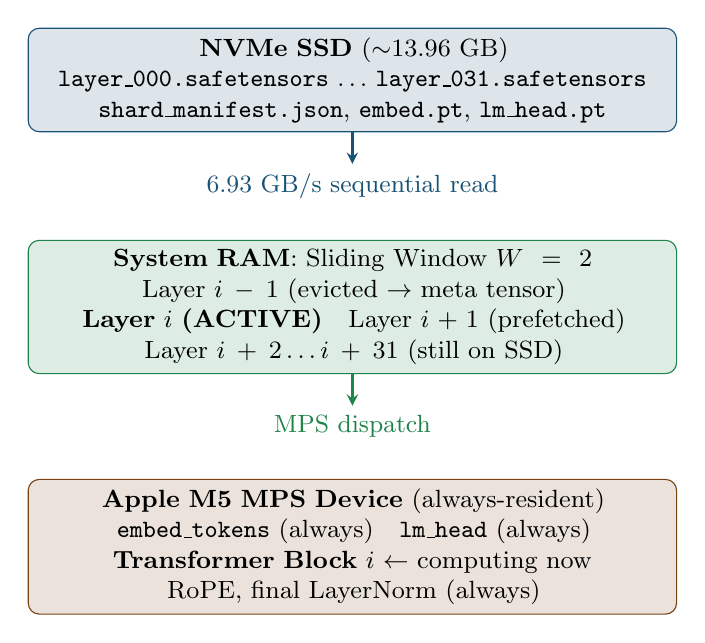
\begin{tikzpicture}[
  node distance=0.8cm,
  box/.style={rectangle, rounded corners, draw, minimum width=8cm,
              text width=8cm, align=center, minimum height=1.2cm, font=\small},
  arrow/.style={->, >=stealth, thick}
]

% SSD Box
\node[box, fill=ssdblue!15, draw=ssdblue] (ssd) {
  \textbf{NVMe SSD} ($\sim$13.96 GB)\\
  \texttt{layer\_000.safetensors} $\ldots$ \texttt{layer\_031.safetensors}\\
  \texttt{shard\_manifest.json}, \texttt{embed.pt}, \texttt{lm\_head.pt}
};

% Arrow
\node[below=0.4cm of ssd] (arrow1) {\textcolor{ssdblue}{\small 6.93 GB/s sequential read}};
\draw[arrow, ssdblue] (ssd) -- (arrow1);

% RAM Box
\node[box, below=0.4cm of arrow1, fill=ramgreen!15, draw=ramgreen] (ram) {
  \textbf{System RAM}: Sliding Window $W=2$\\
  Layer $i-1$ (evicted $\rightarrow$ meta tensor)\\
  \textbf{Layer $i$ (ACTIVE)}\quad Layer $i+1$ (prefetched)\\
  Layer $i+2 \ldots i+31$ (still on SSD)
};

% Arrow
\node[below=0.4cm of ram] (arrow2) {\textcolor{ramgreen}{\small MPS dispatch}};
\draw[arrow, ramgreen] (ram) -- (arrow2);

% MPS Box
\node[box, below=0.4cm of arrow2, fill=mpsbrown!15, draw=mpsbrown] (mps) {
  \textbf{Apple M5 MPS Device} (always-resident)\\
  \texttt{embed\_tokens} (always)\quad \texttt{lm\_head} (always)\\
  \textbf{Transformer Block $i$} $\leftarrow$ computing now\\
  RoPE, final LayerNorm (always)
};

\end{tikzpicture}
\caption{\swlp{} architecture: three residency tiers (NVMe SSD $\rightarrow$ RAM
sliding window $\rightarrow$ MPS device). A background thread prefetches layer
$i+W$ while block $i$ computes; each block is evicted to a zero-byte meta tensor
immediately after its forward pass.}
\label{fig:architecture}
\end{figure}

\subsection{Shard Format}
\label{subsec:shard}

\swlp{} shards the model into per-layer \texttt{.safetensors}
\cite{huggingface2022safetensors} files via \texttt{shard\_model\_by\_layer()}.
The function streams weights one tensor at a time from the HuggingFace checkpoint
without loading the full model into RAM, so a 44~GB model can be sharded on a
16~GB machine. Shard creation is a one-time operation ($\sim$5~minutes for 7B):

\begin{lstlisting}
shards/mistral-7b/
  embed.pt                # embedding + positional encoding
  lm_head.pt              # language model head
  layer_000.safetensors   # transformer block 0
  ...
  layer_031.safetensors   # transformer block 31
  shard_manifest.json     # metadata: model_id, num_layers, layer_weight_mb
\end{lstlisting}

\subsection{StreamingScheduler}
\label{subsec:scheduler}

\texttt{StreamingScheduler} maintains a sliding window of $W$ layers, with a
background thread prefetching layer $i+W$ from SSD while layer $i$ computes on
MPS. After each layer completes, the block is immediately evicted via
\texttt{to\_empty} (parameters become zero-byte \texttt{meta} tensors), keeping
MPS memory at $\approx$1 layer and preventing unified-memory pressure.
Algorithm~\ref{alg:scheduler} gives the per-token sweep; scheduler selection
(Table~\ref{tab:schedulers}) is automatic.

\begin{algorithm}[htbp]
\caption{StreamingScheduler: one decode-step layer sweep}
\label{alg:scheduler}
\begin{algorithmic}[1]
\Require sharded model on disk, window depth $W$, layer count $L$
\State load \{embed, lm\_head, norms\} to device \Comment{resident, done once}
\State spawn prefetch of layers $0 \ldots W{-}1$ into RAM \Comment{background threads}
\State $x \gets \text{embed}(\text{input tokens})$
\For{$i \gets 0$ to $L-1$}
  \State wait until layer $i$ resident in RAM
  \State move layer $i$ weights $\to$ MPS device
  \State spawn async prefetch of layer $i{+}W$ from disk \Comment{overlaps with line 8}
  \State $x \gets \text{block}_i(x)$ \Comment{MPS compute}
  \State evict layer $i \to$ meta (zero-byte) \Comment{free RAM immediately}
\EndFor
\State \Return $\text{lm\_head}(\text{norm}(x))$
\end{algorithmic}
\end{algorithm}

\begin{table}[htbp]
\centering
\caption{Scheduler selection logic}
\label{tab:schedulers}
\begin{tabular}{@{}lll@{}}
\toprule
\textbf{Hardware} & \textbf{Shards} & \textbf{Scheduler} \\
\midrule
Any & Yes & StreamingScheduler (NVMe$\rightarrow$RAM$\rightarrow$device) \\
CUDA & No & SWLPScheduler (CUDA async DMA) \\
MPS/CPU & No & ThreadedScheduler (Python threads) \\
\bottomrule
\end{tabular}
\end{table}

\subsection{Architecture Adapters}
\label{subsec:adapters}

\swlp{} supports major decoder architectures via \texttt{ArchAdapter}. A new
architecture is added by implementing the protocol and registering its model-type
string; the adapter handles position encodings, causal masks, and KV-cache types
while the streaming engine stays architecture-agnostic. Critically, the adapter
reads \texttt{head\_dim} directly from the HuggingFace config, so models with an
explicit \texttt{head\_dim} (partial RoPE, \eg{} Mistral-Small-24B) work
correctly: the exact case where AirLLM crashes.

\subsection{KV Cache Management}
\label{subsec:kv}

\swlp{} provides a three-tier KV cache manager: (1) \textbf{Device}: on-MPS
tensors up to a configurable budget; (2) \textbf{Host}: CPU RAM offload with
async copy; (3) \textbf{Disk}: zlib-compressed spill to NVMe. zlib compression
is bit-exact (lossless) but yields only $\sim$1.1$\times$ on high-entropy FP16 KV
activations at $\sim$3\% generate-time overhead, so its value is host/disk tiering
of cold layers, not raw ratio. An optional INT4 KV tier is available as opt-in
lossy acceleration (not used in the FP16 experiments reported here).

\subsection{Interactive and Speculative Tiers}
\label{subsec:tiers}

\texttt{SpeculativeRunner} extends the base runner with a prompt-lookup n-gram
drafter that reduces full-layer sweeps on repetitive completions while remaining
bit-identical to greedy \swlp{} (\S\ref{subsec:spec}). For interactive speed where
near-lossless INT8 quantization is acceptable, \texttt{MlxRunner} uses native
Apple MLX at $\sim$16~tok/s for Mistral-7B int8 (\S\ref{subsec:mlx}). All runners
are interchangeable through a single \texttt{build\_runner()} factory.

% ═══════════════════════════════════════════════════════════════════════════
% IV. THEORETICAL ANALYSIS
% ═══════════════════════════════════════════════════════════════════════════
\section{Theoretical Analysis}
\label{sec:theory}

\subsection{I/O-Bound Throughput Ceiling}
\label{subsec:ceiling}

Let $B$ be the SSD sequential read bandwidth (GB/s) and $M$ the bytes streamed per token, i.e.\ the on-disk per-layer shard total (GB,
FP16; \eg{} 13.96~GB for Mistral-7B, Table~\ref{tab:models}). Each generated token requires one full sweep through all transformer
blocks, so the minimum wall time per token and the maximum throughput are:
\begin{equation}
t_{\text{sweep}} = \frac{M}{B} \quad \text{(s)},
\qquad
\max \text{ tok/s} = \frac{1}{t_{\text{sweep}}} = \frac{B}{M}.
\label{eq:maxtok}
\end{equation}
For the M5 ($B = 6.93$~GB/s measured) and Mistral-7B ($M = 13.96$~GB):
\begin{equation}
\max \text{ tok/s (cold)} = \frac{6.93}{13.96} = 0.496 \text{ tok/s}.
\label{eq:mistral7b}
\end{equation}
For Mistral-Small-24B ($M = 44.0$~GB):
\begin{equation}
\max \text{ tok/s (cold)} = \frac{6.93}{44.0} = 0.158 \text{ tok/s}.
\label{eq:mistral24b}
\end{equation}

These are \textbf{hard physical ceilings}. The measured cold-cache throughput of
0.174~tok/s reaches 35.1\% of the 0.496~tok/s ceiling; the remaining 64.9\% is
per-layer compute and scheduling overhead that cannot be hidden. Crucially, no
single-stream scheduler can exceed Eq.~\ref{eq:maxtok}: this is the feasibility
boundary referenced throughout the paper.

\subsection{Memory Model}
\label{subsec:memory}

\begin{equation}
\text{RAM}_{\text{peak}} = \text{resident} + W \times \text{layer} + \text{kv}.
\label{eq:ram}
\end{equation}
For Mistral-7B with $W=2$ (resident $\approx$ 500~MB, layer $\approx$ 436~MB),
$\text{RAM}_{\text{peak}} \approx 1{,}372$~MB (measured: 1{,}210~MB, within 12\%).
For Mistral-Small-24B, $\text{RAM}_{\text{peak}} \approx 3{,}100$~MB (measured:
3{,}760~MB; KV cache accounts for the difference). RAM is governed by $W$ and the
per-layer size, \emph{not} by total model depth, the property that lets a 44~GB
model run in under 4~GB.

\subsection{Prefetch Efficiency}
\label{subsec:prefetch}

\begin{equation}
t_{\text{io}} = \frac{436 \text{ MB}}{6{,}930 \text{ MB/s}} \approx 63 \text{ ms},
\qquad
t_{\text{compute}} \approx \frac{150 \text{ ms}}{32 \text{ layers}} \approx 4.7 \text{ ms}.
\label{eq:tio}
\end{equation}
Since $t_{\text{io}} \gg t_{\text{compute}}$ (63~ms vs.\ 4.7~ms), \swlp{} cannot
fully hide I/O at cold-SSD speed: prefetch overlaps only a bounded fraction of
each read behind compute, so any advantage over AirLLM~2.11.0 comes from
scheduling and a smaller resident footprint (\S\ref{subsec:prefetch-note}), not
from beating the ceiling.

% ═══════════════════════════════════════════════════════════════════════════
% V. EXPERIMENTAL SETUP
% ═══════════════════════════════════════════════════════════════════════════
\section{Experimental Setup}
\label{sec:setup}

\subsection{Hardware}
\label{subsec:hardware}

\begin{table}[htbp]
\centering
\caption{Hardware specifications (measured via \texttt{phase0\_hardware\_check.py})}
\label{tab:hardware}
\begin{tabular}{@{}ll@{}}
\toprule
\textbf{Component} & \textbf{Specification} \\
\midrule
Machine & Apple MacBook (M5) \\
Unified Memory & 16 GB LPDDR5X (153 GB/s) \\
Compute & Apple M5 (MPS) \\
Storage & NVMe SSD, 6.93 GB/s seq.\ read, 4.48 GB/s seq.\ write \\
OS & macOS 26.x Tahoe (Darwin 25.4.0) \\
Python & 3.13.13 \\
\bottomrule
\end{tabular}
\end{table}

\subsection{Software}
\label{subsec:software}

\begin{table}[htbp]
\centering
\caption{Software versions (pinned for reproducibility)}
\label{tab:software}
\begin{tabular}{@{}ll@{}}
\toprule
\textbf{Package} & \textbf{Version} \\
\midrule
torch & 2.12.0 \\
transformers & 5.8.1 \\
accelerate & 1.13.0 \\
safetensors & 0.7.0 \\
airllm & 2.11.0 \\
mlx & 0.31.2 \\
\bottomrule
\end{tabular}
\end{table}

\subsection{Models}
\label{subsec:models}

\begin{table}[htbp]
\centering
\caption{Models evaluated}
\label{tab:models}
\begin{tabular}{@{}llll@{}}
\toprule
\textbf{Model} & \textbf{Layers} & \textbf{FP16 Size} & \textbf{Tested By} \\
\midrule
Mistral-7B-Instruct-v0.2 & 32 & 13.96 GB & \swlp{} + AirLLM \\
Qwen2.5-14B-Instruct & 48 & 26.4 GB & \swlp{} only \\
Mistral-Small-24B-Instruct & 40 & $\sim$44 GB & \swlp{} only$^\dagger$ \\
\bottomrule
\end{tabular}
\\[0.3em]
{\small $^\dagger$AirLLM crashes with a RoPE dimension error on 24B
(\texttt{head\_dim}=128 but AirLLM computes 160).}
\\[0.2em]
{\small \textbf{FP16 Size} is the measured on-disk total of the streamed per-layer
shards (\eg{} Mistral-7B $= 32 \times 436$~MB $= 13.96$~GB), \ie{} the bytes that
move per token and enter Eq.~\ref{eq:maxtok}; the always-resident embedding and
\texttt{lm\_head} are excluded, so it sits slightly below a naive
parameters$\times 2$ estimate.}
\end{table}

\subsection{Benchmark Protocol}
\label{subsec:protocol}

\textbf{Workload.} Three prompts of increasing length: P1 (minimal, ``What is
2+2?''), P2 (medium, transformer attention), P3 (long, the solar system).
\textbf{Decoding.} \texttt{max\_new\_tokens=32}, \texttt{temperature=0} (greedy),
\texttt{seed=42}, FP16 throughout. Greedy + fixed seed makes generation
deterministic, so quality equivalence is a byte-level check rather than a
statistical one. \textbf{Timing.} 1 warmup run (discarded) + 2 timed runs, median
reported; both systems are measured in the \emph{same} process invocation on the
\emph{same} prompts with the \emph{same} cache mode. \textbf{Cache control.} In
cold mode the OS page cache is dropped (\texttt{sudo purge}) immediately before
\emph{each} timed run, after warmup, so MPS kernels and the tokenizer stay warm
but the weights are cold; \texttt{cache\_state} is recorded in every JSON result.
\textbf{Reporting convention.} Cold-cache is the headline streaming number;
warm-cache is reported as a clearly-labelled upper bound. Because the
absolute SWLP throughput was historically inflated by warm cache (see
Table~\ref{tab:superseded} and Appendix~\ref{app:methodology}), each table below
states its cache state explicitly.

% ═══════════════════════════════════════════════════════════════════════════
% VI. RESULTS
% ═══════════════════════════════════════════════════════════════════════════
\section{Results}
\label{sec:results}

Sections~\ref{subsec:quality}--\ref{subsec:fp8} form the core characterization
(quality, throughput, latency, peak memory, the model ladder, and two negative
results); Sections~\ref{subsec:spec}--\ref{subsec:mlx} report three secondary,
optional tiers (speculative decoding, batched streaming, and the native-MLX
interactive backend) that complement but are not central to the lossless-streaming
thesis.

\subsection{Quality Equivalence}
\label{subsec:quality}

Two \swlp{} runs under greedy decoding produce byte-identical output, verified by
the CI test suite (\texttt{test\_quality\_equivalence.py}). Table~\ref{tab:quality}
shows \swlp{} and AirLLM completions; both produce factually correct answers, and
token-level differences arise only from FP16 rounding between PyTorch/MPS (\swlp{})
and MLX (AirLLM), not from factual errors. By construction \swlp{} computes the
same FP16 weights on the same device as a full in-RAM forward pass, so it
introduces zero quality loss relative to non-streaming FP16.

\begin{table}[htbp]
\centering
\caption{Quality comparison: Mistral-7B FP16, greedy, 32 tokens}
\label{tab:quality}
\small
\begin{tabular}{@{}p{1.2cm}p{5.3cm}p{5.3cm}@{}}
\toprule
\textbf{Prompt} & \textbf{\swlp{} Output} & \textbf{AirLLM Output} \\
\midrule
P1 & ``\ldots{} The answer is 4, but the way we arrive at that\ldots'' & ``2+2 is equal to 4. This is a basic arithmetic problem.'' \\
P2 & ``Transformer attention is a self-attention mechanism used in the Transformer model\ldots'' & ``\ldots{} allows a model to focus on different parts of the input sequence\ldots'' \\
P3 & ``The solar system is a vast and complex collection of celestial bodies that orbit\ldots'' & ``\ldots{} all orbiting around a central star, the Sun.\ldots'' \\
\bottomrule
\end{tabular}
\end{table}

\subsection{Throughput: Mistral-7B, Warm Cache}
\label{subsec:throughput}

Table~\ref{tab:throughput} and Figure~\ref{fig:bars} report the warm-cache
head-to-head. \swlp{} is $\sim$2.5$\times$ faster than AirLLM~2.11.0 on average; the P3
outlier (4.0$\times$) is AirLLM degrading under the macOS memory compressor after
two consecutive 13.96~GB page-cache sweeps, a failure mode \swlp{} avoids because
immediate eviction keeps the resident set small (see \S\ref{subsec:prefetch-note}
for the version and mechanism caveat).

\begin{table}[htbp]
\centering
\caption{Throughput (tok/s): Mistral-7B FP16, warm-cache, $W=2$ (higher is better)}
\label{tab:throughput}
\begin{tabular}{@{}lccc@{}}
\toprule
\textbf{Prompt} & \textbf{\swlp{}} & \textbf{AirLLM} & \textbf{Speedup} \\
\midrule
P1 (minimal) & 0.202 & 0.099 & 2.04$\times$ \\
P2 (medium) & 0.214 & 0.102 & 2.10$\times$ \\
P3 (long) & 0.213 & 0.053 & 4.02$\times$$^\ddagger$ \\
\midrule
\textbf{Average} & \textbf{0.210} & \textbf{0.085} & \textbf{2.47$\times$} \\
\bottomrule
\end{tabular}
\\[0.3em]
{\small $^\ddagger$AirLLM P3 degraded due to macOS memory-compressor activation
after two consecutive 13.96~GB page-cache sweeps.}
\end{table}

\begin{figure}[htbp]
\centering
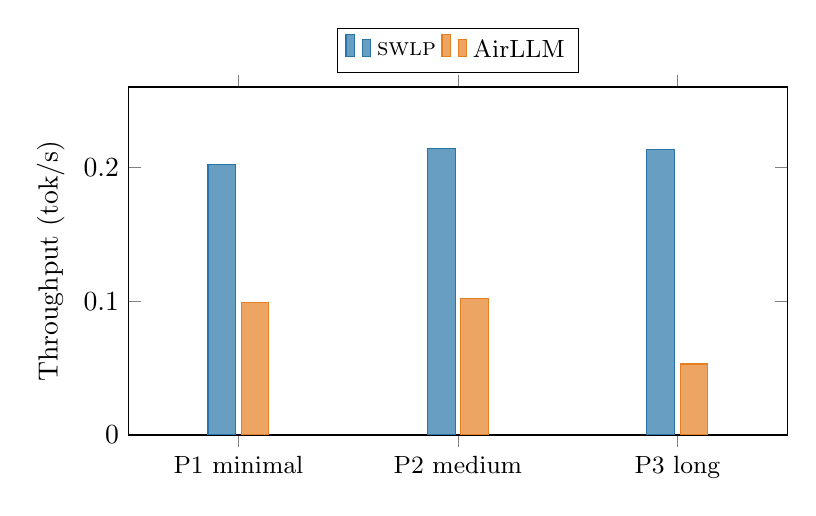
\begin{tikzpicture}
\begin{axis}[
  width=0.82\linewidth, height=6cm,
  ybar, bar width=10pt,
  symbolic x coords={P1 minimal, P2 medium, P3 long},
  xtick=data, x tick label style={font=\small},
  ymin=0, ymax=0.26,
  ylabel={Throughput (tok/s)},
  legend style={at={(0.5,1.04)}, anchor=south, legend columns=2, font=\small},
  enlarge x limits=0.25,
  % per-bar value labels omitted; exact figures are in the adjacent table.
]
\addplot[fill=swlpblue!70, draw=swlpblue] coordinates {(P1 minimal,0.202) (P2 medium,0.214) (P3 long,0.213)};
\addplot[fill=airllmorange!70, draw=airllmorange] coordinates {(P1 minimal,0.099) (P2 medium,0.102) (P3 long,0.053)};
\legend{\swlp{}, AirLLM}
\end{axis}
\end{tikzpicture}
\caption{Warm-cache throughput, Mistral-7B FP16 ($W=2$). \swlp{} sustains
$\sim$0.21~tok/s across prompts; AirLLM is roughly half and collapses on P3 under
memory-compressor pressure.}
\label{fig:bars}
\end{figure}

\subsection{Time to First Token and Peak RAM: Warm Cache}
\label{subsec:ttft}

\swlp{} keeps embeddings, \texttt{lm\_head}, and norms permanently resident and
prefetches the window, so the first token emerges far sooner than AirLLM, which
pays a full 32-layer disk sweep before token one (Table~\ref{tab:ttft}). \swlp{}
also uses less RAM at every prompt (Table~\ref{tab:ram}) because it evicts each
block to a meta tensor immediately, whereas AirLLM's MLX runtime retains larger
intermediate buffers.

\begin{minipage}[t]{0.48\linewidth}
\centering
\captionof{table}{TTFT (ms): warm cache (lower is better)}
\label{tab:ttft}
\begin{tabular}{@{}lccc@{}}
\toprule
\textbf{Prompt} & \textbf{\swlp{}} & \textbf{AirLLM} & \textbf{Adv.} \\
\midrule
P1 & 4{,}707 & 10{,}434 & 2.22$\times$ \\
P2 & 6{,}015 & 9{,}383 & 1.56$\times$ \\
P3 & 5{,}145 & 20{,}584 & 4.00$\times$ \\
\midrule
\textbf{Avg} & \textbf{5{,}289} & \textbf{13{,}467} & \textbf{2.55$\times$} \\
\bottomrule
\end{tabular}
\end{minipage}\hfill
\begin{minipage}[t]{0.48\linewidth}
\centering
\captionof{table}{Peak RAM (GB): warm cache (lower is better)}
\label{tab:ram}
\begin{tabular}{@{}lccc@{}}
\toprule
\textbf{Prompt} & \textbf{\swlp{}} & \textbf{AirLLM} & \textbf{Adv.} \\
\midrule
P1 & 0.79 & 1.83 & 2.32$\times$ \\
P2 & 0.97 & 1.70 & 1.75$\times$ \\
P3 & 1.21 & 1.52 & 1.26$\times$ \\
\midrule
\textbf{Peak} & \textbf{1.21} & \textbf{1.83} & \textbf{1.51$\times$} \\
\bottomrule
\end{tabular}
\end{minipage}

\subsection{Cold-Cache Measurements: Mistral-7B}
\label{subsec:cold}

Cold-cache measurements (page cache cleared via \texttt{sudo purge} before every
timed run; the \texttt{cache\_state} field verified as \texttt{cold} in each JSON
result) were obtained on 2026-05-30 using the cold protocol of
Appendix~\ref{app:reproduction}.

\begin{table}[htbp]
\centering
\caption{\swlp{} cold-cache throughput: Mistral-7B FP16, $W=2$}
\label{tab:cold}
\begin{tabular}{@{}lccc@{}}
\toprule
\textbf{Prompt} & \textbf{TTFT (ms)} & \textbf{tok/s} & \textbf{\% of ceiling$^\S$} \\
\midrule
P1 (minimal) & 6{,}432 & 0.133 & 26.8\% \\
P2 (medium) & 5{,}294 & 0.186 & 37.5\% \\
P3 (long) & 4{,}183 & 0.203 & 40.9\% \\
\midrule
\textbf{Average} & \textbf{5{,}303} & \textbf{0.174} & \textbf{35.1\%} \\
\bottomrule
\end{tabular}
\\[0.3em]
{\small $^\S$Cold ceiling $= 6.93 / 13.96 = 0.496$~tok/s (Eq.~\ref{eq:mistral7b}).
TTFT is reported for completeness but is noisy at $n=2$ and not directly
comparable to the warm TTFT of Table~\ref{tab:ttft} (per-prompt ordering can
invert within run-to-run variance); throughput is the headline cold metric.}
\end{table}

Cold \swlp{} (0.174~tok/s avg) outperforms warm AirLLM (0.085~tok/s avg) by
\textbf{2.05$\times$}. This is deliberately a \emph{conservative} comparison: it
pits \swlp{}'s worst case (cold SSD) against AirLLM's best case (warm cache), so
the advantage is a lower bound, not a cherry-pick. A symmetric cold-vs-cold
AirLLM measurement is deferred (Section~\ref{sec:limitations}). The warm/cold
ratio for \swlp{} is only 1.21$\times$ (MPS dispatch and Python scheduling
dominate, both cache-agnostic), which is itself evidence that \swlp{} is doing
real streaming rather than reading from page cache.

\subsection{Model Ladder: 7B / 14B / 24B Feasibility (RQ1)}
\label{subsec:ladder}

Table~\ref{tab:ladder} and Figure~\ref{fig:ladder} answer RQ1: all three scales
run on the 16~GB M5 with peak RAM far below the model size, while every naive
full-model load OOMs. Measured throughput is reported against each model's own
bandwidth ceiling (Eq.~\ref{eq:maxtok}), which makes the rows comparable despite
their absolute magnitudes differing. The 14B rung reaches the highest fraction of
its ceiling: larger layers amortize fixed per-layer scheduling overhead, so
streaming efficiency \emph{improves} with model size even as absolute throughput
falls.

\begin{table}[htbp]
\centering
\caption{Model ladder: \swlp{} FP16, $W=2$, warm cache. ``Ceiling'' is
$B/M$ (Eq.~\ref{eq:maxtok}); naive full-model load OOMs on 16~GB in every case}
\label{tab:ladder}
\begin{tabular}{@{}lcccccc@{}}
\toprule
\textbf{Model} & \textbf{Params} & \textbf{FP16 size} & \textbf{Ceiling} & \textbf{tok/s} & \textbf{\% ceil.} & \textbf{RAM peak} \\
\midrule
Mistral-7B & 7B & 13.96 GB & 0.496 & 0.210 & 42\% & 1.21 GB \\
Qwen2.5-14B & 14B & 26.4 GB & 0.263 & 0.194 & 74\% & 1.66 GB \\
Mistral-Small-24B & 24B & 44.0 GB & 0.158 & 0.081 & 51\% & 3.76 GB \\
\bottomrule
\end{tabular}
\\[0.3em]
{\small Warm-cache; the Mistral-7B cold-cache figure is 0.174~tok/s (35\% of
ceiling, Table~\ref{tab:cold}). AirLLM runs only 7B (0.085~tok/s) and crashes on
24B; it was not benchmarked on 14B.}
\end{table}

\begin{figure}[htbp]
\centering
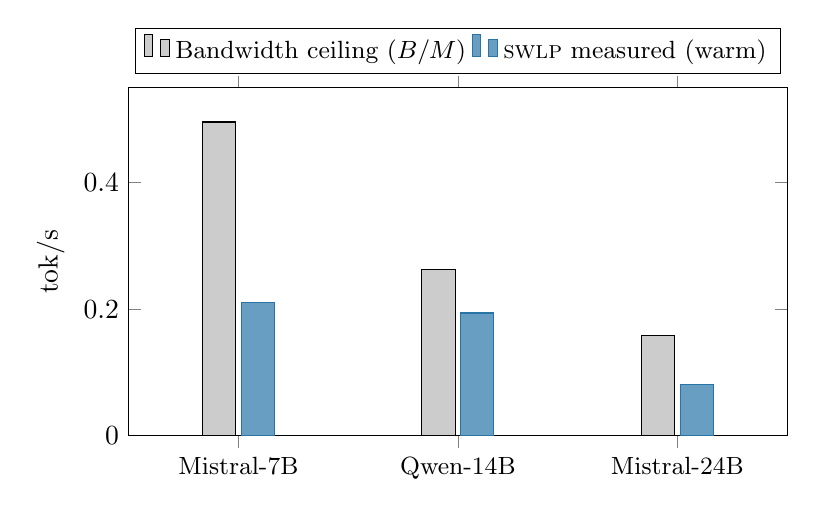
\begin{tikzpicture}
\begin{axis}[
  width=0.82\linewidth, height=6cm,
  ybar, bar width=12pt,
  symbolic x coords={Mistral-7B, Qwen-14B, Mistral-24B},
  xtick=data, x tick label style={font=\small},
  ymin=0, ymax=0.55,
  ylabel={tok/s},
  legend style={at={(0.5,1.04)}, anchor=south, legend columns=2, font=\small},
  enlarge x limits=0.25,
  % per-bar value labels omitted; exact figures are in the adjacent table.
]
\addplot[fill=medgray, draw=black] coordinates {(Mistral-7B,0.496) (Qwen-14B,0.263) (Mistral-24B,0.158)};
\addplot[fill=swlpblue!70, draw=swlpblue] coordinates {(Mistral-7B,0.210) (Qwen-14B,0.194) (Mistral-24B,0.081)};
\legend{Bandwidth ceiling ($B/M$), \swlp{} measured (warm)}
\end{axis}
\end{tikzpicture}
\caption{Model-ladder throughput vs.\ the bandwidth ceiling. Both fall with model
size; measured \swlp{} tracks closest to the ceiling at 14B (74\%), where larger
layers best amortize per-layer overhead.}
\label{fig:ladder}
\end{figure}

\subsection{Window-Size Ablation (RQ3)}
\label{subsec:window}

\begin{table}[htbp]
\centering
\caption{Window-depth sweep: Mistral-7B FP16, M5, end-to-end SWLPRunner.
Early Phase-1 warm-cache harness (16 tokens); absolute throughput is an upper
bound (cf.\ Table~\ref{tab:superseded}), retained here for the \emph{W-trend}}
\label{tab:window}
\begin{tabular}{@{}ccc@{}}
\toprule
\textbf{Window $W$} & \textbf{tok/s} & \textbf{TTFT (ms)} \\
\midrule
2 & \textbf{0.40} & 6 \\
4 & 0.29 & 14 \\
6 & 0.25 & 22 \\
\bottomrule
\end{tabular}
\\[0.3em]
{\small Peak RAM is omitted: in this early Phase-1 harness it was non-monotonic in
$W$ (a measurement artifact), and the authoritative peak-RAM figures appear in
Tables~\ref{tab:ram} and~\ref{tab:ladder}.}
\end{table}

On discrete VRAM, a deeper window hides more I/O and should raise throughput.
On M5 unified memory the opposite holds (Table~\ref{tab:window},
Figure~\ref{fig:window}): throughput is highest at $W=2$ and falls monotonically
with $W$. A larger resident window competes with the OS page cache for the
\emph{same} physical RAM, so extra prefetch depth buys no hidden I/O and instead
raises CPU$\leftrightarrow$GPU memory pressure. (A synthetic pipeline POC with
simulated compute favored larger $W$; the real run inverts this: a concrete
instance of unified memory behaving unlike VRAM, RQ2.) We therefore use $W=2$
throughout.

\begin{figure}[htbp]
\centering
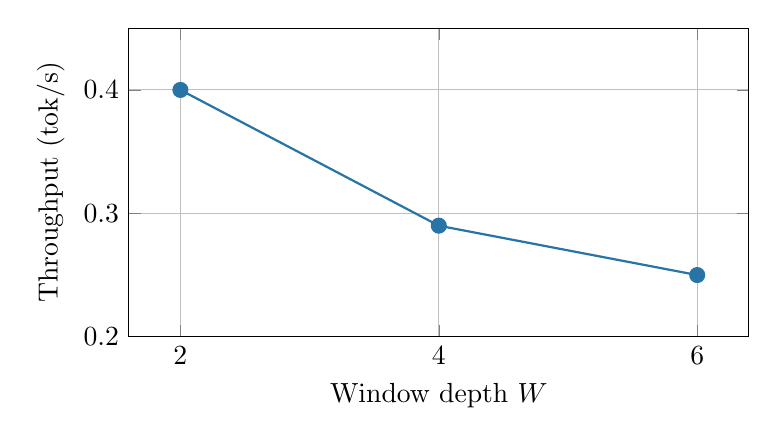
\begin{tikzpicture}
\begin{axis}[
  width=0.78\linewidth, height=5.5cm,
  xlabel={Window depth $W$}, ylabel={Throughput (tok/s)},
  xtick={2,4,6}, ymin=0.2, ymax=0.45,
  grid=major, mark size=2.5pt,
]
\addplot[swlpblue, thick, mark=*] coordinates {(2,0.40) (4,0.29) (6,0.25)};
\end{axis}
\end{tikzpicture}
\caption{Throughput decreases monotonically with window depth on M5 unified
memory, the opposite of the discrete-VRAM intuition. $W=2$ is the operating
point used throughout.}
\label{fig:window}
\end{figure}

\subsection{Negative Result: In-RAM Residency Does Not Help (RQ2, RQ3)}
\label{subsec:residency}

We hypothesized that caching some layers permanently in RAM would cut per-token
disk traffic. On 16~GB it does the reverse (Table~\ref{tab:residency}): locking 17
layers ($17 \times 436$~MB $= 7.4$~GB) starves the page cache for the remaining
streamed shards, triggering the macOS memory compressor and slowing every memory
access process-wide, a 6--12$\times$ regression. The fix is a
\emph{full-model-fit guard}: residency is enabled only when the whole model fits
within 75\% of $(\text{RAM} - 6\,\text{GB})$, which on 16~GB means zero resident
layers for 7B+ and restores full streaming speed. This is a unified-memory-specific
hazard (RQ2): on discrete VRAM, host-resident layers do not contend with GPU
memory the same way.

\begin{table}[htbp]
\centering
\caption{In-RAM residency, Mistral-7B FP16, M5 (warm-cache reference run)}
\label{tab:residency}
\begin{tabular}{@{}lccl@{}}
\toprule
\textbf{Configuration} & \textbf{tok/s} & \textbf{RAM peak} & \textbf{Outcome} \\
\midrule
$W=2$ streaming (0 resident) & 0.505 & 1.47 GB & baseline \\
17 layers MPS-resident & 0.041 & $\sim$9 GB & Metal fragmentation, 12$\times$ slower \\
17 layers CPU-RAM resident & 0.080 & $\sim$9 GB & memory compressor, 6$\times$ slower \\
\texttt{auto} (fit-guard $\to$ 0 resident) & \textbf{0.505} & 1.47 GB & speed restored \\
\bottomrule
\end{tabular}
\end{table}

\subsection{Negative Result: FP8 Storage Does Not Help (RQ3)}
\label{subsec:fp8}

Halving the bytes on disk (per-output-channel-scaled \texttt{float8\_e4m3}, FP16
compute) should halve disk traffic and raise throughput. It does not
(Table~\ref{tab:fp8}): throughput \emph{fell} to 0.86$\times$ (7B) and 0.53$\times$
(14B), even though shard sizes genuinely halved (Mistral 218~MB vs.\ 436~MB; Qwen
275~MB vs.\ 551~MB). The cause is architectural: \swlp{} re-materializes every
layer onto the device on \emph{every} token, so each layer is dequantized
FP8$\to$FP16 on CPU per token, and that dequant costs about as much as the disk
read it replaced. The same per-token dequant also explains the peak-RAM blow-up
in Table~\ref{tab:fp8} (7.34~GB vs.\ 1.47~GB): an FP16 materialization buffer is
allocated per layer on every token and is released less promptly than the
streaming evictor frees it, so the FP8 tier costs \emph{more} memory, not less.
The weight quality held perfectly (the FP8-7B completion is
byte-identical to FP16), but the throughput thesis failed. The lesson:
``store smaller'' helps only if it becomes ``compute faster,'' which on Apple
Silicon means native quantized matmul (\S\ref{subsec:mlx}), not streamed weight
precision tricks. INT4 storage would fail worse still.

\begin{table}[htbp]
\centering
\caption{FP8 weight storage, M5, $W=2$ (warm-cache reference; the result is the
\emph{ratio} under identical conditions). Quality is byte-identical to FP16}
\label{tab:fp8}
\begin{tabular}{@{}lcccc@{}}
\toprule
\textbf{Configuration} & \textbf{Layer size} & \textbf{tok/s} & \textbf{RAM peak} & \textbf{vs FP16} \\
\midrule
Mistral-7B FP16 & 436 MB & 0.505 & 1.47 GB & 1.00$\times$ \\
Mistral-7B FP8 & 218 MB & 0.436 & 7.34 GB & 0.86$\times$ \\
Qwen2.5-14B FP16 & 551 MB & 0.194 & 1.66 GB & 1.00$\times$ \\
Qwen2.5-14B FP8 & 275 MB & 0.102 & 3.60 GB & 0.53$\times$ \\
\bottomrule
\end{tabular}
\end{table}

\subsection{Speculative Decoding (Lossless, Workload-Dependent)}
\label{subsec:spec}

Prompt-lookup n-gram speculation verifies multiple tokens per disk sweep with no
draft model and zero extra RAM. Output is byte-identical to greedy \swlp{}
(Table~\ref{tab:spec}). The speedup is workload-dependent: free-form text has no
recurring n-grams and degrades gracefully to baseline minus a $\sim$7\% drafting
overhead, while repetition-heavy output (long-context QA that quotes its source,
code, structured lists) reaches 4.0 tokens/sweep and 3.29$\times$, exactly the
workloads \swlp{} targets. When the drafter fires, acceptance is 100\%: the
variable is how often a matching n-gram exists, not whether proposals are
accepted.

\begin{table}[htbp]
\centering
\caption{Prompt-lookup speculative decoding, Mistral-7B FP16, M5
(within-run warm-cache baseline 0.505~tok/s; the ratios hold under identical
conditions, cf.\ \S\ref{subsec:cold}). All outputs byte-identical to greedy \swlp{}}
\label{tab:spec}
\begin{tabular}{@{}lcccc@{}}
\toprule
\textbf{Workload} & \textbf{Drafts acc.} & \textbf{tokens/sweep} & \textbf{tok/s} & \textbf{vs baseline} \\
\midrule
Novel free-form & 0 / 0 & 1.03 & 0.471 & 0.93$\times$ \\
Mildly repetitive & 6 / 6 & 1.28 & 0.578 & 1.15$\times$ \\
Repetition-heavy & 35 / 35 & \textbf{4.00} & \textbf{1.66} & \textbf{3.29$\times$} \\
\bottomrule
\end{tabular}
\end{table}

\subsection{Batched Streaming (Column-Wise Execution)}
\label{subsec:batch}

A layer's disk read costs the same whether 1 or $N$ sequences pass through it, so
processing a batch in lockstep amortizes the read across all $N$ (FlexGen's
column-wise execution). Decode-sweep wall time stays essentially flat
($\sim$0.24--0.34~s) from batch 1 to 16, so aggregate throughput scales nearly
linearly (Table~\ref{tab:batch}): batch 16 is $\sim$18.5$\times$ the batch-1 rate,
fully lossless (each row byte-identical to a batch-1 run). Numbers are on
SmolLM2-360M (small layers, modest absolute rates); the \emph{scaling} is
architecture-independent and is the result the conclusion rests on. A 7B/14B
batched re-measurement is pending shard re-download (Section~\ref{sec:limitations}).

\begin{table}[htbp]
\centering
\caption{Batched streaming, SmolLM2-360M FP16, $W=2$, M5}
\label{tab:batch}
\begin{tabular}{@{}rrr@{}}
\toprule
\textbf{Batch} & \textbf{Sweep time (s)} & \textbf{Aggregate tok/s} \\
\midrule
1 & 0.282 & 3.54 \\
2 & 0.326 & 6.13 \\
4 & 0.264 & 15.13 \\
8 & 0.337 & 23.73 \\
16 & 0.243 & \textbf{65.75} \\
\bottomrule
\end{tabular}
\end{table}

\subsection{The Interactive Tier: Native MLX (Lossy by Choice)}
\label{subsec:mlx}

Streaming buys feasibility, not interactivity. For interactive use, \swlp{} ships
an \texttt{MlxRunner} using native Apple MLX quantized matmul
(Table~\ref{tab:mlx}). MLX int8 on Mistral-7B runs at 16~tok/s with a
\emph{byte-identical} completion to FP16 (a near-lossless interactive default), while int4 trades a small wording drift for $\sim$1.7$\times$ more speed.
Quantization doubles as a memory dial: 14B int8 ($\sim$14~GB) OOMs on 16~GB, but
14B int4 ($\sim$7~GB) fits and runs at 13.8~tok/s. The two runners span the
quality/speed/feasibility surface from one factory: streaming for lossless
big-model feasibility, MLX for interactive speed.

\begin{table}[htbp]
\centering
\caption{Native MLX interactive tier vs.\ FP16 streaming, M5}
\label{tab:mlx}
\begin{tabular}{@{}llccl@{}}
\toprule
\textbf{Model} & \textbf{Backend} & \textbf{tok/s} & \textbf{vs FP16} & \textbf{Quality} \\
\midrule
Mistral-7B & \swlp{} FP16 stream & 0.21 & 1$\times$ & reference \\
Mistral-7B & MLX int8 & \textbf{16.0} & 76$\times$ & byte-identical \\
Mistral-7B & MLX int4 & 27.9 & 133$\times$ & minor drift \\
Qwen2.5-14B & \swlp{} FP16 stream & 0.194 & 1$\times$ & reference \\
Qwen2.5-14B & MLX int8 & n/a & n/a & OOM ($>$16 GB) \\
Qwen2.5-14B & MLX int4 & 13.8 & 71$\times$ & minor drift \\
\bottomrule
\end{tabular}
\\[0.3em]
{\small \swlp{} streaming rows are warm-cache references (\S\ref{subsec:cold};
0.21 / 0.194~tok/s); against the authoritative \emph{cold} 0.174~tok/s the MLX
int8 gap on Mistral-7B widens to $\sim$92$\times$. MLX RAM is under-reported
(\S\ref{sec:limitations}).}
\end{table}

% ═══════════════════════════════════════════════════════════════════════════
% VII. DISCUSSION
% ═══════════════════════════════════════════════════════════════════════════
\section{Discussion}
\label{sec:discussion}

\subsection{When Streaming Wins}
\label{subsec:when}
\swlp{} is the right tool when (1) the model is too large to load even after
quantization; (2) lossless FP16 quality is required (perplexity, sensitivity
analysis, fine-tuning evaluation, deterministic outputs); and (3) a latency of one
token every few seconds is acceptable (research evaluation, background or batch
generation). For interactive conversation ($<$1~s/token) the MLX tier
(\S\ref{subsec:mlx}) is appropriate. \swlp{} occupies a specific niche:
\emph{feasibility at full precision}, not interactive speed.

\subsection{Why the Negative Results Are the Interesting Ones}
\label{subsec:why-negative}
Two intuitive optimizations both failed, and they failed for the \emph{same}
reason: the bottleneck on M5 is not disk bandwidth in isolation but the
per-token re-materialization of weights through a memory pool shared with the OS.
In-RAM residency (\S\ref{subsec:residency}) and FP8 storage (\S\ref{subsec:fp8})
each attacked disk traffic, and each was either neutralized (FP8: CPU dequant
costs what the read saved) or actively harmful (residency: page-cache starvation
$\to$ memory compressor). What surprised us most was the window-size inversion
(\S\ref{subsec:window}): more prefetch depth made things \emph{slower}. Together
these results sharpen the claim of the paper: on unified memory, the path to
speed is not smarter streaming but leaving streaming behind for native quantized
compute. This is why the feasibility boundary (Eq.~\ref{eq:maxtok}) is a contribution
rather than a caveat.

\subsection{Streaming vs.\ Quantization}
\label{subsec:tradeoff}
The fundamental trade is: streaming pays in latency, quantization pays in quality.
At its authoritative cold 0.174~tok/s (0.21~tok/s warm), \swlp{} is
$\sim$92$\times$ slower than MLX int8 ($\sim$76$\times$ at the warm upper bound),
but its output is
provably identical to a full FP16 run (same weights, same computation, same
device). INT8 introduces small, model-dependent rounding error at every matmul.
For applications where FP16 accuracy is load-bearing, that difference matters; for
chat, it usually does not.

\subsection{AirLLM Version and Mechanism Caveat}
\label{subsec:prefetch-note}
We pin AirLLM~2.11.0 for a reproducible baseline and run its MLX class
\texttt{AirLLMLlamaMlx}. AirLLM's documented async prefetch is enabled by default
for its \emph{separate} PyTorch \texttt{AirLLMLlama2} class, not the MLX class we
use; we did not separately profile whether \texttt{AirLLMLlamaMlx} overlaps I/O
with compute, so we do \emph{not} attribute the measured throughput gap to a
prefetch-vs-no-prefetch difference, and a prefetch-controlled re-run is future
work (\S\ref{sec:limitations}). Two advantages are mechanism-independent and hold
regardless of how that resolves: the RAM-efficiency gap (immediate per-block
eviction vs.\ AirLLM's larger retained buffers, Table~\ref{tab:ram}) and the
architecture-coverage gap (explicit \texttt{head\_dim}, which lets \swlp{} run the
24B that crashes AirLLM).

% ═══════════════════════════════════════════════════════════════════════════
% VIII. THREATS TO VALIDITY
% ═══════════════════════════════════════════════════════════════════════════
\section{Threats to Validity}
\label{sec:threats}

We organize threats along the standard four axes.

\textbf{Internal validity.} The dominant confound is OS page-cache state, which can
make a ``streaming'' run read from RAM and report an impossible throughput
(Appendix~\ref{app:methodology}). We mitigate with a provenance-stamped cold
protocol that drops the cache before each timed run and records the verified
\texttt{cache\_state}; a run that cannot drop the cache is labelled warm, never
cold. The headline streaming number is cold-cache.

\textbf{External validity.} All experiments run on one M5 (16~GB) machine, so
results may not generalize to other Apple Silicon SKUs or to discrete VRAM. The
M5 16~GB is, however, representative of the consumer configuration the work
targets, and the bandwidth bound (Eq.~\ref{eq:maxtok}) is hardware-parametric. The
CUDA path is implemented but unbenchmarked (Section~\ref{sec:limitations}).

\textbf{Construct validity.} Throughput is measured at 32 output tokens; because
throughput is disk-bound rather than KV-bound at this scale, it is expected to be
stable for longer outputs, but long-context KV streaming is not yet validated.
TTFT definitions differ between harnesses (prefill-inclusive vs.\ argmax-only), so
we do not compare TTFT \emph{across} the model ladder, only within a harness.

\textbf{Conclusion validity.} Greedy + fixed seed makes each configuration
deterministic, so quality equivalence is a byte-level check rather than a sampled
statistic; throughput is the median of $\ge$2 timed runs after a discarded warmup.
Sample sizes are small (single machine, two timed runs), so absolute numbers carry
run-to-run variance even though the SWLP-vs-AirLLM \emph{direction} is robust
across every run we collected.

\textbf{Baseline coverage.} HF~Accelerate disk-offload is implemented in the
harness but not benchmarked here, so it is omitted from the results tables; the
naive HF/MLX full-model load is reported as the relevant fact (OOM on 16~GB).
The AirLLM comparison is cold-\swlp{} vs.\ warm-AirLLM, an intentionally
conservative pairing (\S\ref{subsec:cold}); a symmetric cold-AirLLM run is future
work.

% ═══════════════════════════════════════════════════════════════════════════
% IX. LIMITATIONS
% ═══════════════════════════════════════════════════════════════════════════
\section{Limitations}
\label{sec:limitations}

We state the limitations of this study plainly:

\begin{enumerate}[leftmargin=2em]
  \item \textbf{Single hardware platform.} Only the M5 16~GB is measured. The
    NVIDIA CUDA path (async DMA via \texttt{SWLPScheduler}) is implemented but not
    benchmarked due to hardware unavailability; a discrete-GPU column (\eg{}
    MX230 RAM$\to$VRAM streaming) is the most important missing evaluation.
  \item \textbf{Sub-interactive throughput is inherent.} Single-stream lossless
    FP16 streaming cannot exceed $B/M$ (Eq.~\ref{eq:maxtok}); this is a property
    of the regime, not a tuning gap. Interactive speed requires the MLX tier
    (lossy) or batching.
  \item \textbf{Short context.} All runs use 32 output tokens. Long-context KV
    streaming (4{,}096+ tokens) is designed but not yet measured at scale.
  \item \textbf{Unbenchmarked baselines.} oLLM (\texttt{flash-attn} fails on
    Apple Silicon) and HF~Accelerate disk-offload are not yet measured head-to-head.
  \item \textbf{Single-session 14B/24B runs.} The 14B and 24B rungs were each
    measured in one session under matching config; they are not yet re-validated
    across sessions.
  \item \textbf{Batched numbers are on a small model.} The linear batch scaling is
    demonstrated on SmolLM2-360M; a 7B/14B batched measurement awaits shard
    re-download.
  \item \textbf{MLX memory under-reporting.} \texttt{psutil} RSS under-reports
    MLX's wired/memory-mapped GPU memory, so MLX RAM figures are a floor.
\end{enumerate}

% ═══════════════════════════════════════════════════════════════════════════
% X. ETHICAL CONSIDERATIONS
% ═══════════════════════════════════════════════════════════════════════════
\section{Ethical Considerations}
\label{sec:ethics}

This work studies inference \emph{efficiency} and introduces no new model weights,
no training data, and no human-subjects component; all experiments use publicly
released open-weight models (Mistral, Qwen) under their respective licenses. The
primary societal effect is positive: lowering the hardware barrier lets
researchers, students, and practitioners run full-precision models on commodity
laptops, improving reproducibility and access without a cloud account or a
data-center GPU. The dual-use surface is minimal (efficient inference of
already-public models does not expand misuse capability beyond what those models
already permit), and the lossless-by-default stance avoids the silent quality
degradation that can make quantized deployments behave unpredictably. We note an
energy trade-off: streaming sustains low memory but runs long, so per-token energy
on a battery device is higher than a resident quantized run; we therefore present
the MLX tier as the appropriate choice for routine interactive use.

% ═══════════════════════════════════════════════════════════════════════════
% XI. CONCLUSION AND FUTURE WORK
% ═══════════════════════════════════════════════════════════════════════════
\section{Conclusion and Future Work}
\label{sec:conclusion}

\swlp{} shows that lossless FP16 inference of models larger than system RAM is
practical on consumer Apple Silicon. Streaming transformer blocks from SSD through
a sliding window yields a $\sim$2.5$\times$ throughput advantage over
AirLLM~2.11.0 at $\sim$1.5$\times$ less RAM and $\sim$2.5$\times$
lower TTFT on Mistral-7B FP16 (warm cache), and even cold it beats warm
AirLLM~2.11.0 by 2.05$\times$. A 44~GB model otherwise unrunnable on 16~GB streams at 0.081~tok/s in
3.76~GB. The bandwidth bound $\text{tok/s}\le B/M$ gives a closed-form ceiling that
explains why all single-stream lossless streamers are sub-interactive, and our two
negative results (FP8 storage, in-RAM residency) show the ceiling cannot be moved
by precision or residency tricks under per-token re-materialization. The honest
takeaway is a map of the design space, not a speed record.

\textbf{Future work:} (1) the NVIDIA MX230 CUDA DMA column; (2) a symmetric
cold-cache AirLLM and an oLLM comparison once \texttt{flash-attn} builds on Apple
Silicon; (3) long-context KV-cache streaming at 4{,}096+ tokens with the
host/disk tiers; (4) a 7B/14B batched re-measurement; and (5) quantitative
logit-level equivalence on Mistral-7B beyond the byte-level check.

% ═══════════════════════════════════════════════════════════════════════════
% REPRODUCIBILITY
% ═══════════════════════════════════════════════════════════════════════════
\section{Reproducibility}
\label{sec:repro}

Every result in this paper is reproducible from the public repository. We
summarize the essentials here; exact commands are in
Appendix~\ref{app:reproduction} and the integrity protocol in
Appendix~\ref{app:methodology}.

\begin{itemize}[leftmargin=2em]
  \item \textbf{Code:} open source at
    \url{https://github.com/Rishav-Upadhaya/SWLP}; install from source
    (\texttt{git clone} then \texttt{bash scripts/bootstrap.sh};
    Appendix~\ref{app:reproduction}), including the full benchmark harness,
    provenance scripts, and a 154-test CI suite.
  \item \textbf{Determinism:} greedy decoding, \texttt{temperature=0},
    \texttt{seed=42}; quality equivalence is byte-level and CI-checked.
  \item \textbf{Provenance:} every benchmark JSON embeds git commit, platform,
    library versions, hardware (chip, RAM, measured SSD bandwidth), and verified
    \texttt{cache\_state}.
  \item \textbf{Versions:} pinned (Table~\ref{tab:software}); AirLLM 2.11.0.
  \item \textbf{Cache protocol:} \texttt{--cold} drops the page cache before each
    timed run; warm runs are labelled, never passed off as cold.
\end{itemize}

\noindent\textbf{Reproducibility checklist.}
\begin{itemize}[leftmargin=2em,nosep]
  \item[$\boxtimes$] Code and install path public and versioned.
  \item[$\boxtimes$] Exact model IDs, sizes, and shard format specified
    (Tables~\ref{tab:models},~\ref{tab:tiers}).
  \item[$\boxtimes$] Hardware and software fully specified
    (Tables~\ref{tab:hardware},~\ref{tab:software}).
  \item[$\boxtimes$] Decoding hyperparameters and seed reported
    (\S\ref{subsec:protocol}).
  \item[$\boxtimes$] Per-run provenance and cache state recorded; cited JSON files
    listed (Data and Code Availability section).
  \item[$\boxtimes$] Number of runs, warmup, and aggregation stated
    (\S\ref{subsec:protocol}).
  \item[$\square$] Multi-platform (CUDA) results: deferred
    (Section~\ref{sec:limitations}).
\end{itemize}

% ═══════════════════════════════════════════════════════════════════════════
% DATA AND CODE AVAILABILITY
% ═══════════════════════════════════════════════════════════════════════════
\section*{Data and Code Availability}
\addcontentsline{toc}{section}{Data and Code Availability}
\label{sec:data}

The \swlp{} library is open source at \url{https://github.com/Rishav-Upadhaya/SWLP}
(install from source; see Appendix~\ref{app:reproduction}). Benchmark data with full provenance live in the
\texttt{benchmarks/} directory. The specific JSON files cited here are:

\begin{itemize}[leftmargin=2em]
  \item Warm-cache Mistral-7B \swlp{}: \texttt{airllm\_vs\_swlp\_20260521T111258Z.json}
  \item Warm-cache AirLLM Mistral-7B: \texttt{airllm\_vs\_swlp\_20260521T111304Z.json}
  \item Cold-cache Mistral-7B \swlp{}: \texttt{airllm\_vs\_swlp\_20260530T064840Z.json}
  \item Warm-cache Mistral-Small-24B \swlp{}: \texttt{airllm\_vs\_swlp\_20260521T121612Z.json}
\end{itemize}

% ═══════════════════════════════════════════════════════════════════════════
% ACKNOWLEDGMENTS
% ═══════════════════════════════════════════════════════════════════════════
\section*{Acknowledgments}
\addcontentsline{toc}{section}{Acknowledgments}

This research received no external funding. The author thanks the open-source
communities behind PyTorch, HuggingFace Transformers, and Apple MLX for the
foundational tools that made this work possible.

% ═══════════════════════════════════════════════════════════════════════════
% REFERENCES
% ═══════════════════════════════════════════════════════════════════════════
\begin{thebibliography}{16}

\bibitem{jiang2023mistral}
A. Q. Jiang \etal, ``Mistral 7B,'' \textit{arXiv preprint arXiv:2310.06825}, 2023.
\url{https://arxiv.org/abs/2310.06825}

\bibitem{llama32024}
Meta AI, ``Llama 3: Open Foundation and Fine-Tuned Chat Models,'' 2024.
\url{https://ai.meta.com/blog/meta-llama-3/}

\bibitem{qwen2024}
Qwen Team, ``Qwen2.5 Technical Report,'' \textit{arXiv preprint arXiv:2412.15115}, 2024.
\url{https://arxiv.org/abs/2412.15115}

\bibitem{frantar2023gptq}
E. Frantar, S. Ashkboos, T. Hoefler, and D. Alistarh, ``GPTQ: Accurate
Post-Training Quantization for Generative Pre-trained Transformers,''
\textit{Proc. ICLR}, 2023. \url{https://arxiv.org/abs/2210.17323}

\bibitem{lin2023awq}
J. Lin \etal, ``AWQ: Activation-aware Weight Quantization for LLM Compression and
Acceleration,'' \textit{arXiv preprint arXiv:2306.00978}, 2023.
\url{https://arxiv.org/abs/2306.00978}

\bibitem{gerganov2023llama}
G. Gerganov \etal, ``llama.cpp,'' GitHub: ggerganov/llama.cpp, 2023.
\url{https://github.com/ggerganov/llama.cpp}

\bibitem{guo2023airllm}
L. Guo, ``AirLLM: Running 70B LLM Inference on a Single 4GB GPU,'' GitHub:
lyogavin/airllm, 2023. \url{https://github.com/lyogavin/Anima/tree/main/air_llm}

\bibitem{alizadeh2023llmflash}
K. Alizadeh \etal, ``LLM in a Flash: Efficient Large Language Model Inference with
Limited Memory,'' \textit{arXiv preprint arXiv:2312.11514}, 2023.
\url{https://arxiv.org/abs/2312.11514}

\bibitem{sheng2023flexgen}
Y. Sheng \etal, ``FlexGen: High-Throughput Generative Inference of Large Language
Models with a Single GPU,'' \textit{Proc. ICML}, pp.\ 31094--31116, 2023.
\url{https://arxiv.org/abs/2303.06865}

\bibitem{rajbhandari2021zero}
S. Rajbhandari \etal, ``ZeRO-Infinity: Breaking the GPU Memory Wall for Extreme
Scale Deep Learning,'' \textit{Proc. SC}, 2021.
\url{https://arxiv.org/abs/2104.07857}

\bibitem{song2023powerinfer}
Y. Song \etal, ``PowerInfer: Fast Large Language Model Serving with a
Consumer-grade GPU,'' \textit{arXiv preprint arXiv:2312.12456}, 2023.
\url{https://arxiv.org/abs/2312.12456}

\bibitem{huang2025edgellm}
M. Huang \etal, ``EdgeLLM: CPU-FPGA Heterogeneous Edge Accelerator for LLMs,''
\textit{IEEE Trans. Circuits Syst. I}, 2025. \url{https://arxiv.org/abs/2407.14385}

\bibitem{leviathan2023fast}
Y. Leviathan, M. Kalman, and Y. Matias, ``Fast Inference from Transformers via
Speculative Decoding,'' \textit{Proc. ICML}, pp.\ 19274--19286, 2023.
\url{https://arxiv.org/abs/2211.17192}

\bibitem{chen2023speculative}
C. Chen \etal, ``Accelerating Large Language Model Decoding with Speculative
Sampling,'' \textit{arXiv preprint arXiv:2302.01318}, 2023.
\url{https://arxiv.org/abs/2302.01318}

\bibitem{huggingface2022safetensors}
HuggingFace, ``safetensors,'' GitHub, 2022.
\url{https://github.com/huggingface/safetensors}

\bibitem{ollm2025}
oLLM Contributors, ``oLLM: LLM Inference for Large-Context Offline Workloads,''
GitHub: Mega4alik/ollm, 2025. \url{https://github.com/Mega4alik/ollm}

\end{thebibliography}

% ═══════════════════════════════════════════════════════════════════════════
% APPENDICES
% ═══════════════════════════════════════════════════════════════════════════
\appendix

\section{Reproduction Commands}
\label{app:reproduction}

\subsection{Environment Setup}
\begin{lstlisting}
git clone https://github.com/Rishav-Upadhaya/SWLP.git
cd SWLP
bash scripts/bootstrap.sh       # creates .venv, installs swlp[dev]
source .venv/bin/activate
pip install airllm==2.11.0      # benchmark-only, not in pyproject.toml
\end{lstlisting}

\subsection{Hardware Check}
\begin{lstlisting}
python scripts/phase0_hardware_check.py
# Reports SSD read/write GB/s, MPS matmul speed, MLX availability.
# Expected on M5 16GB: SSD read ~ 6.5--6.9 GB/s.
\end{lstlisting}

\subsection{Shard Mistral-7B (One-Time)}
\begin{lstlisting}
swlp download --model mistral-7b
# Streams weights from HuggingFace to shards/mistral-7b/.
# ~5 minutes on M5. No full-model RAM load required.
\end{lstlisting}

\subsection{Warm Benchmark (\swlp{} vs AirLLM)}
\begin{lstlisting}
python scripts/compare_airllm_swlp.py --models 7b --runs 2
# ~55 minutes total. JSON saved to benchmarks/airllm_vs_swlp_<ts>.json.
\end{lstlisting}

\subsection{Cold Benchmark (True SSD Streaming, Requires sudo)}
\begin{lstlisting}
# SWLP-only first (no AirLLM, faster):
sudo .venv/bin/python scripts/compare_airllm_swlp.py \
  --models 7b --cold --skip-airllm --runs 2

# Full 3-way cold (SWLP + AirLLM):
sudo .venv/bin/python scripts/compare_airllm_swlp.py \
  --models 7b --cold --runs 2
\end{lstlisting}

\subsection{Quality Equivalence and Test Suite}
\begin{lstlisting}
pytest tests/test_quality_equivalence.py -v
python scripts/quality_equivalence.py \
  --model unsloth/mistral-7b-instruct-v0.2 --shard-dir shards/mistral-7b
pytest                  # 154 tests, all pass
ruff check src/         # zero errors
\end{lstlisting}

\section{Benchmark Methodology and Integrity}
\label{app:methodology}

\subsection{The Page-Cache Trap}
The OS page cache holds recently read pages in RAM. After one full sweep, all
shard files are cached, so a second sweep reads from RAM, not SSD, yielding
$\sim$3--10$\times$ higher throughput. This silently confounds
warmup-plus-timed-run protocols.

\textbf{Worked example of the bug.} An earlier harness reported \textbf{0.505~tok/s}
for Mistral-7B. The cold-SSD ceiling is $6.93/13.96 = 0.496$~tok/s
(Eq.~\ref{eq:mistral7b}); 0.505 exceeds it, which is physically impossible for
streaming from disk: the run was reading page-cached shards from RAM. Only
once we controlled cache state did the honest cold number (0.174~tok/s) emerge.

\subsection{The Cold Protocol}
Both harnesses take \texttt{--cold}, which drops the cache before \emph{each} timed
run (after warmup, so MPS kernels and the tokenizer stay warm; only the weights
are cold). The mechanism is \texttt{purge} on macOS (needs \texttt{sudo}) and
\texttt{sync} + \texttt{drop\_caches} on Linux (needs root). If the cache cannot be
dropped, the drop routine returns the string \texttt{warm (purge needs sudo \ldots)},
which is recorded verbatim as the run's \texttt{cache\_state}, so a warm run is
never mislabelled as cold.

\subsection{Fair Head-to-Head Rules}
\begin{enumerate}[leftmargin=2em]
  \item \textbf{Same harness, same run.} Both systems measured in one process
    invocation, on the same prompts, with the same \texttt{cache\_mode}.
  \item \textbf{Same cache state for both.} \texttt{--cold} drops the cache before
    both timed runs.
  \item \textbf{Median of $\ge$2 timed runs}, 1 warmup discarded; prompt set reported.
  \item \textbf{Same precision tier.} FP16-vs-FP16 only for the headline.
\end{enumerate}

\subsection{The Three Superseded Numbers}
For the record, the pre-audit Mistral-7B $W=2$ FP16 throughput figures and their
provenance (the reconciliation that motivated the cold protocol):

\begin{table}[htbp]
\centering
\caption{Superseded Mistral-7B $W=2$ FP16 throughput figures}
\label{tab:superseded}
\footnotesize
\begin{tabular}{@{}llll@{}}
\toprule
\textbf{tok/s} & \textbf{Source} & \textbf{Conditions} & \textbf{Verdict} \\
\midrule
0.422 & \texttt{benchmarks/phase3.json} & 1 run, 1 prompt, cache uncontrolled & superseded \\
0.502 / 0.505 & \texttt{phase3\_baselines.py} & warmup $\rightarrow$ warm cache & upper bound, not cold \\
0.210 & \texttt{compare\_airllm\_swlp.py} & 3-prompt median, partially warm & closest to honest (warm) \\
\midrule
\textbf{0.174} & \texttt{compare\_airllm\_swlp.py --cold} & 3-prompt median, cold cache & \textbf{authoritative} \\
\bottomrule
\end{tabular}
\end{table}

\end{document}
